
 \newpage
\subsection{SPI-out}
This chapter will describe the SPI-output module. An overview of the module can be seen in Fig. \ref{spi_out}.

\begin{figure}[H]
\centering
\captionsetup{justification=centering}
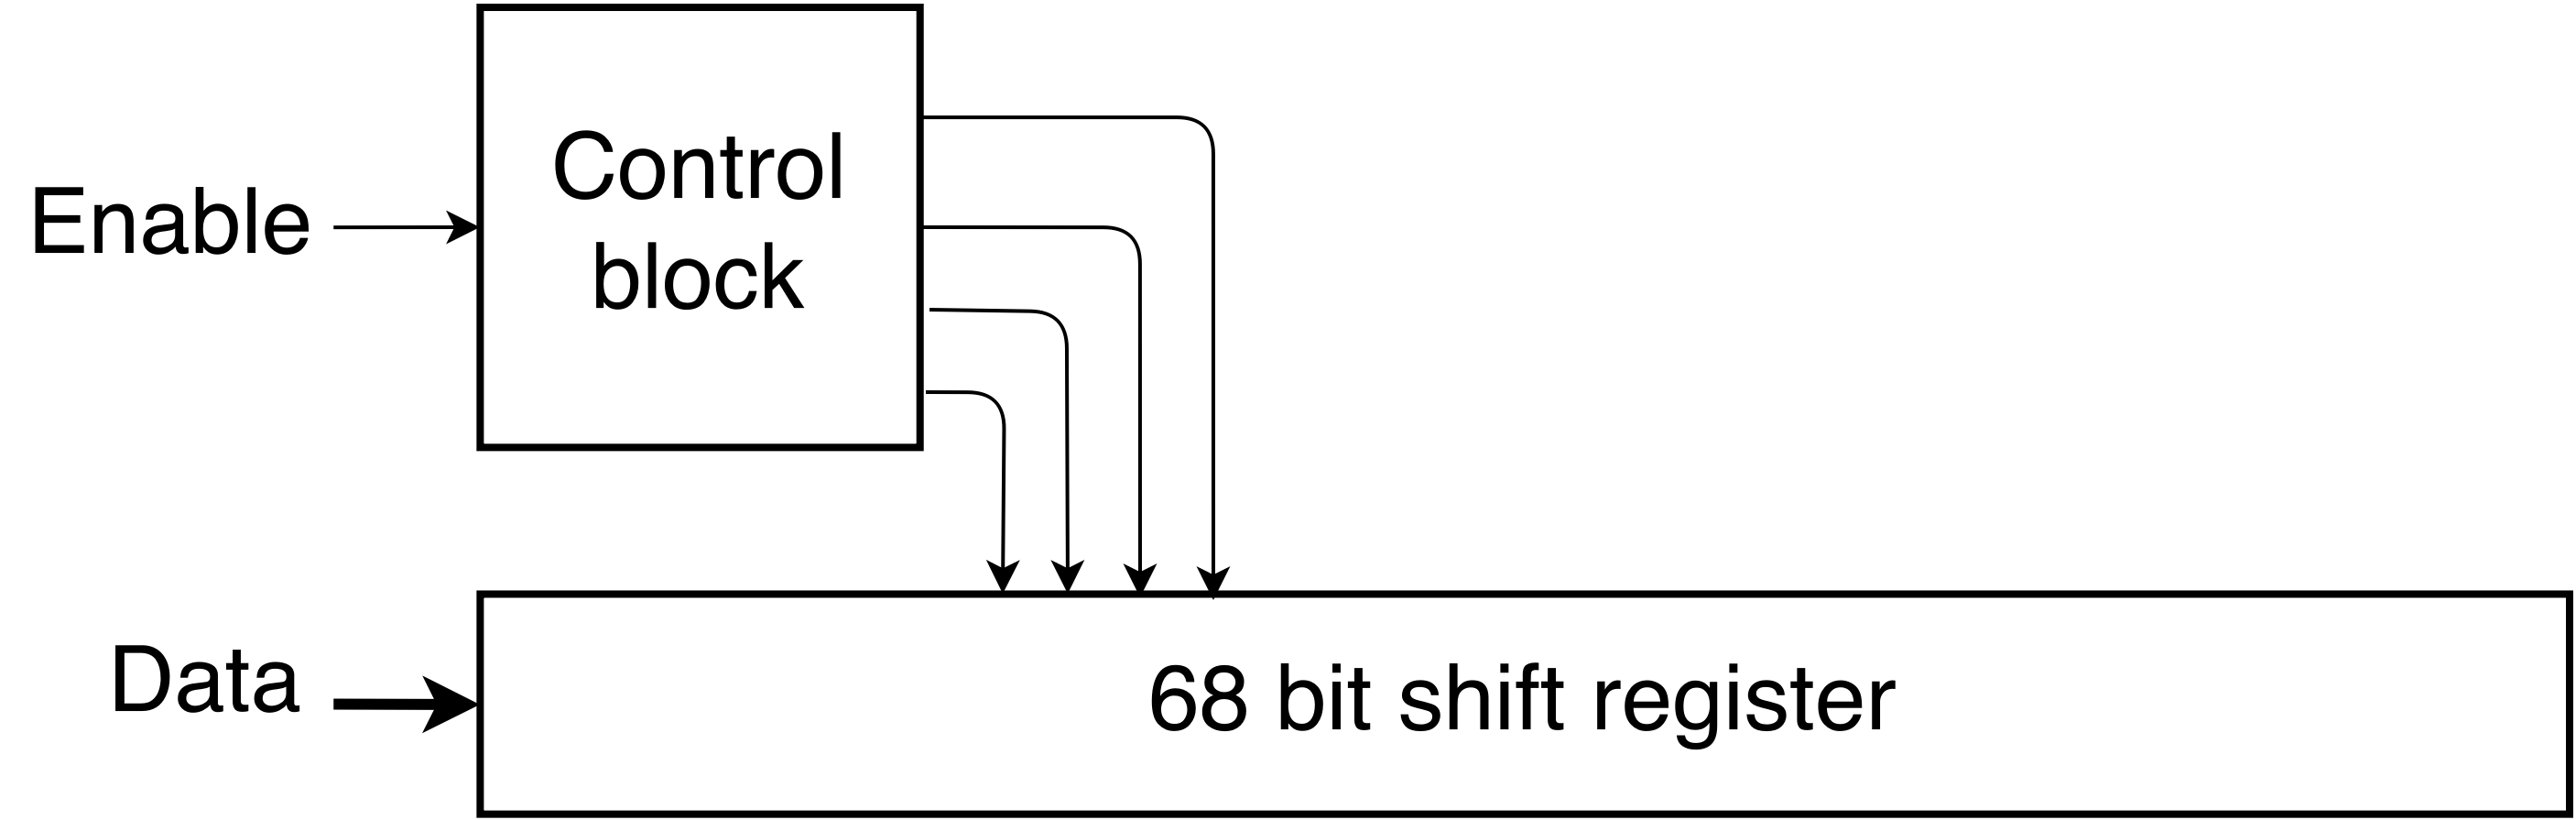
\includegraphics[scale=0.15]{../figures/spi_out.png}
\caption{SPI-out overview}
\label{spi_out}
\end{figure}

\subsubsection{Shift register}
The major component is a 68-bit shift register, for the four 17-bit words, where each cell in the register contains one D flip-flop and one multiplexer. The schematic for a cell can be seen in Fig. \ref{mux_dff}.

\begin{figure}[H]
\centering
\captionsetup{justification=centering}
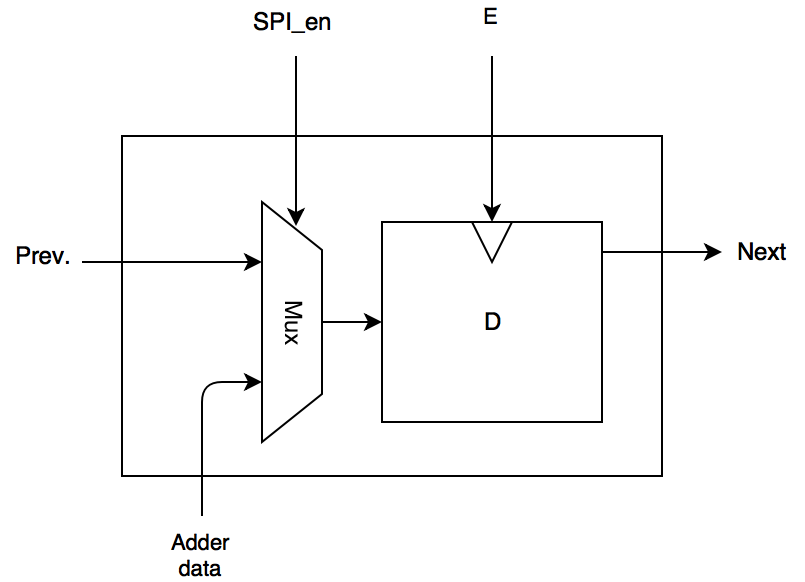
\includegraphics[scale=0.35]{../figures/MUX_DFF.png}
\caption{Shift register cell}
\label{mux_dff}
\end{figure}

\newpage

\subsubsection{Control logic}
The control logic is needed to load the long shift register with the correct data. Since the adder is built in such a way that it executes all the four additions as fast as it can after the SPI enable signal goes high, the output from one addition will only be available for one system clock cycle. This means that we need to quickly grab the data and put it in the correct place.
 
Our implementation uses a pulse generator, a 2-bit counter, a decoder to select what 17-bit part of the shift register to load, and some multiplexers to select if to clock the register on the spi clock or on the enable signals from the decoder. The pulse generator is triggered by the spi enable signal and creates a pulse that is four system clock cycles long. This is to only allow the counter to increment four times, and also to clip the pulse from the last decoder output. As can be seen in Fig. \ref{spi_out} the last output of the decoder is also fed back to the enable of the counter through an inverter. This prevents a possible glitch that is generated on E1 when the counter starts over, which would reload the section of the shift register containing the first sum. \\

\begin{figure}[H]
\centering
\captionsetup{justification=centering}
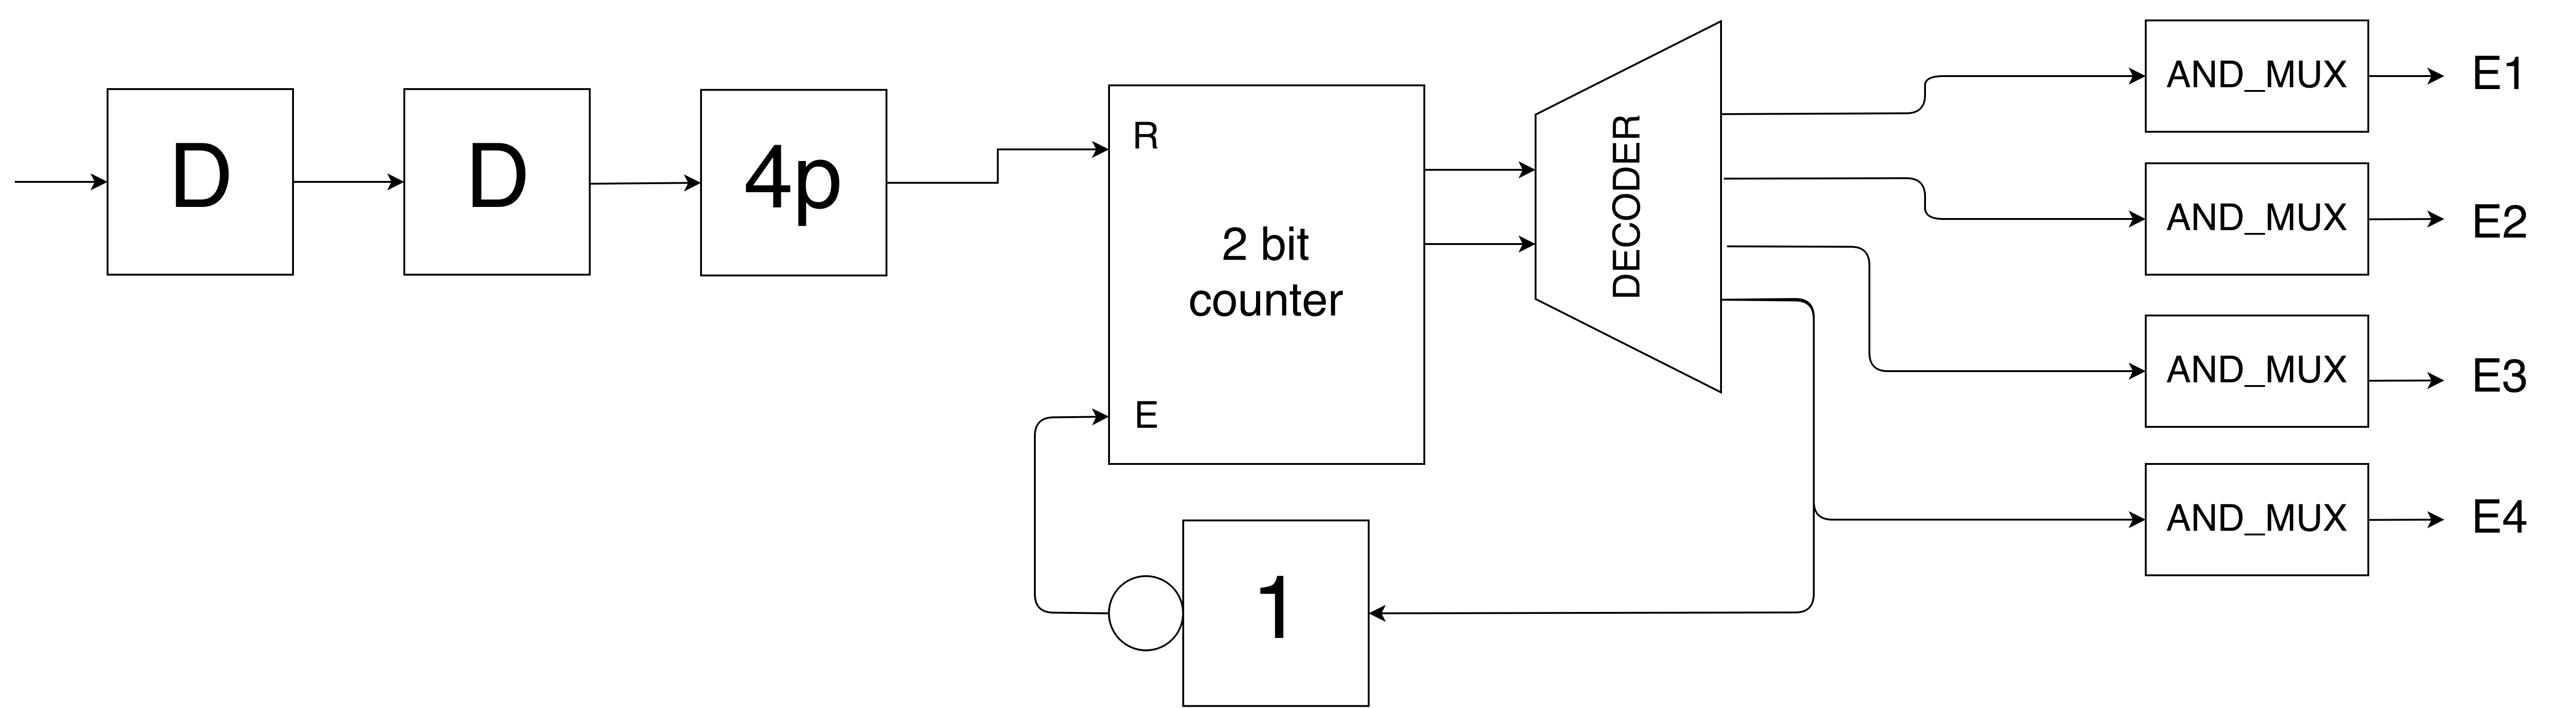
\includegraphics[scale=0.075]{../figures/spi_control.png}
\caption{Control logic for SPI-output}
\label{spi_out}
\end{figure}

\raggedright As can be seen to the left in Fig. \ref{spi_out}, there are two D flip-flops in the beginning. They are needed to sync the SPI enable signal with the data from the adder as the data is delayed by two system clock cycles.\\
To the right there are four enable signals: E1, E2, E3, E4. Each one of those signals enables a specific part of the shift register. If SPI enable is low, all of the signals would be equal to the SPI clock so that data can be shifted out. Otherwise, if the SPI enable signal is high and, for example, E1 is high, the 17-bit part of the shift register corresponding to the sum of the first addition would be loaded with the output from the adder. \\
As each of the enable signals has a high fan out they all need a buffer which can be seen in Fig. \ref{and_mux}.

\begin{figure}[H]
\centering
\captionsetup{justification=centering}
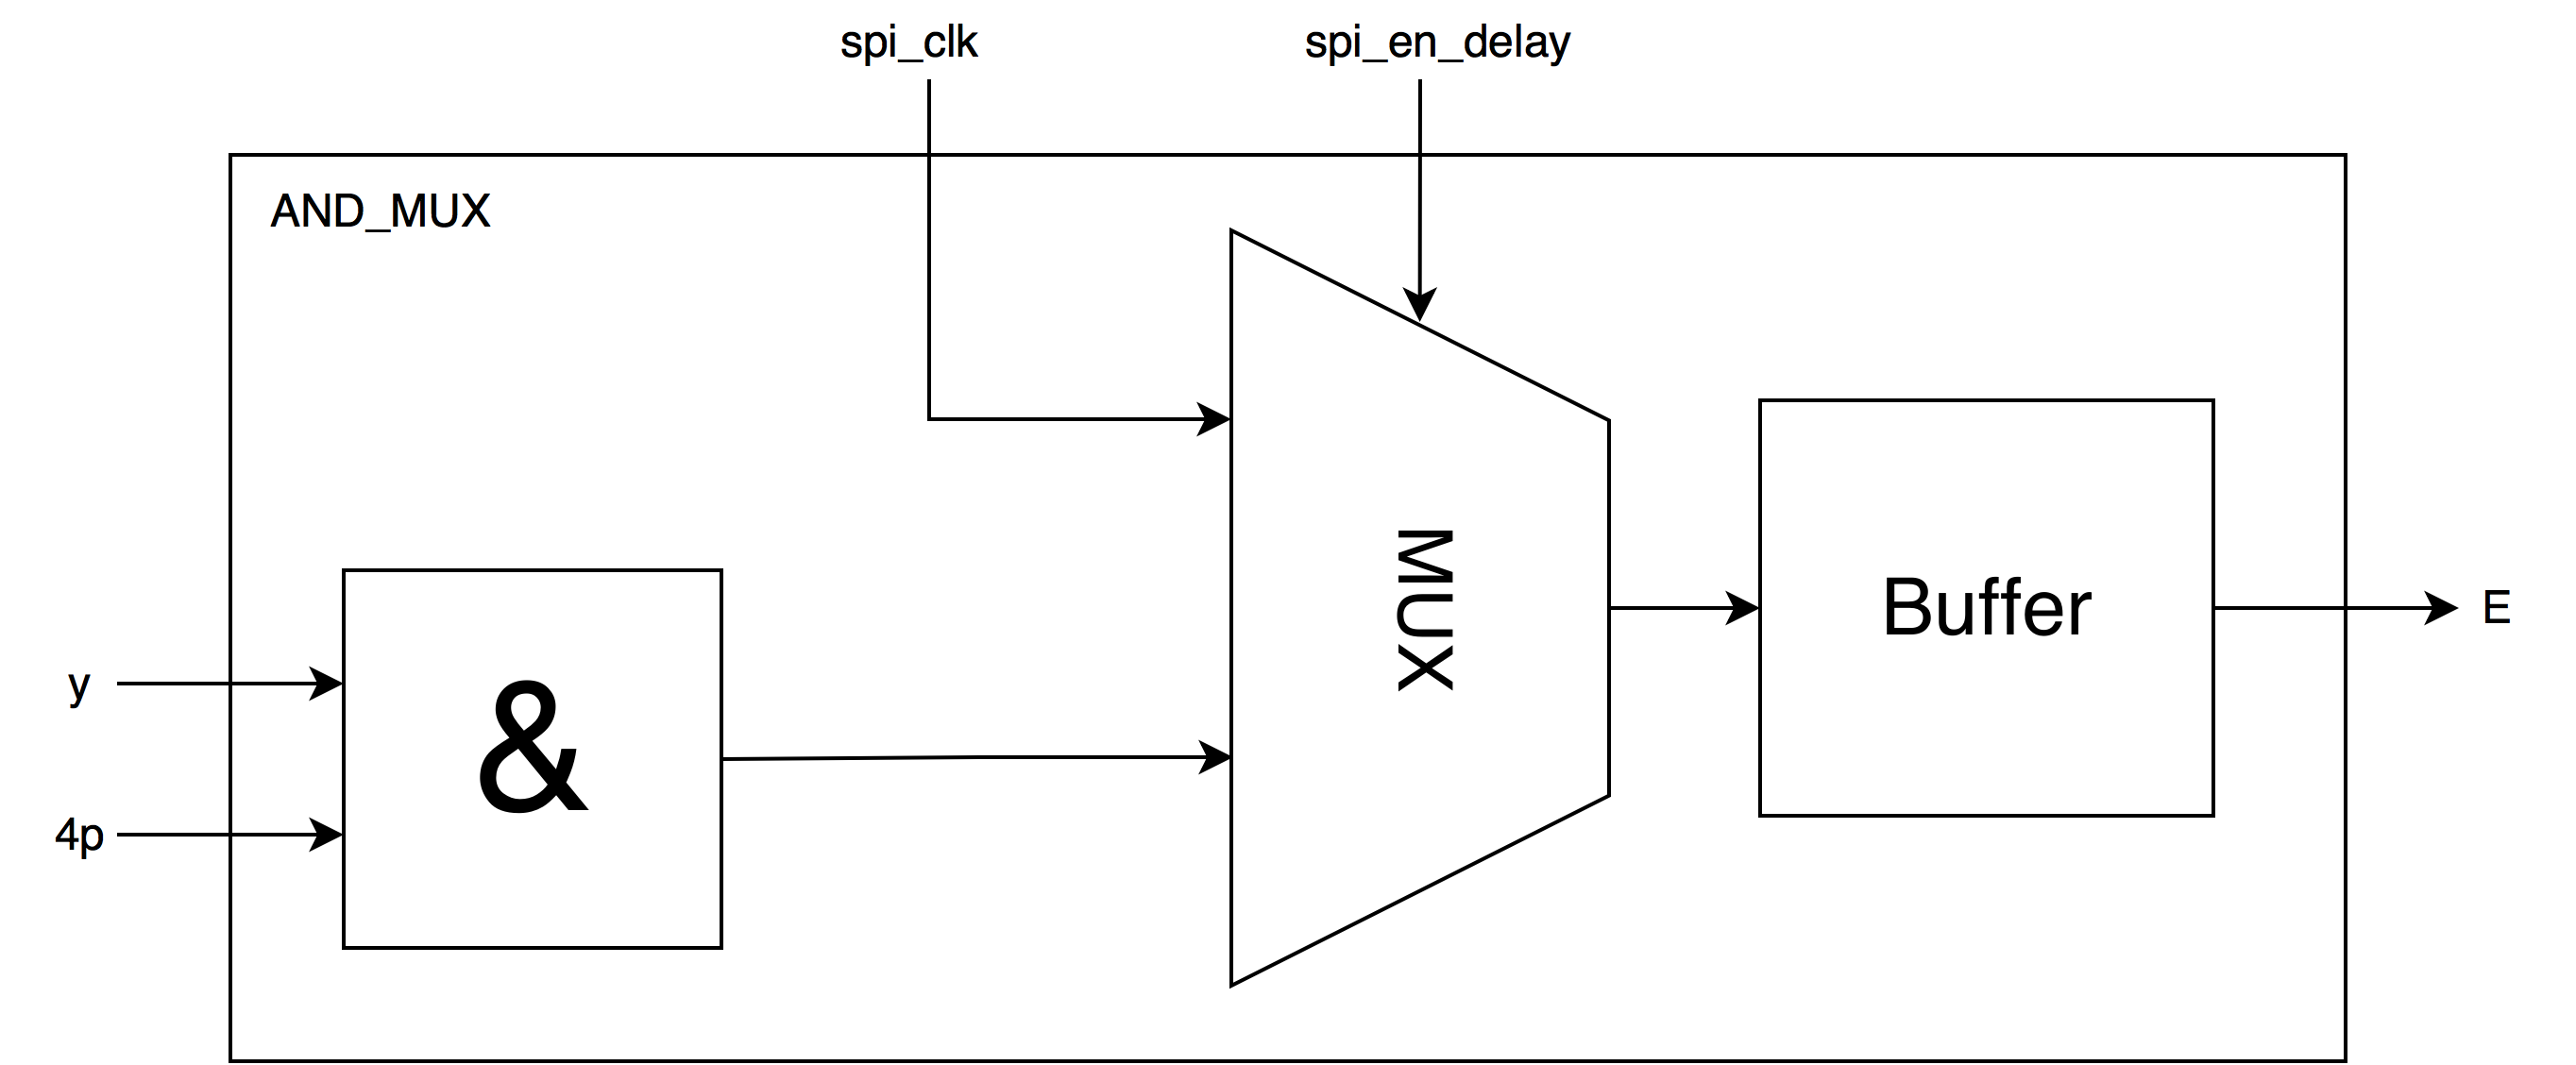
\includegraphics[scale=0.1]{../figures/AND_MUX_ny.png}
\caption{Functional block containing an AND and a MUX.}
\label{and_mux}
\end{figure}




